\section{Time-frequency analysis}

Analysis of the collected data from the thermal camera was done in the time-frequency domain. For this a wavelet transformation of the temperature trace was computed in order to look for specific frequency content in the data. 

Wavelet transformation is practical when looking for signals of lower frequencies compared to the normal Fourier analysis, because of the bigger resolution in the frequency content. Another drawback of the Fourier transform is the loss of time information, which is preserved with the wavelet transformation.\cite{geyer2004}

%Both a discrete wavelet transformation (DWT) and the continuous wavelet transformation (CWT) can be used, but the CWT has better resolution, why this was used for computing the frequency content of the data.\cite{geyer2004} 

The CWT is using a variable sized region windowing technique. Long time intervals are used where low frequency information is computed and short time intervals are used where high frequency information is computed. This is represented in \figref{fig:sigToWave}.

\begin{figure}[H]
	\centering	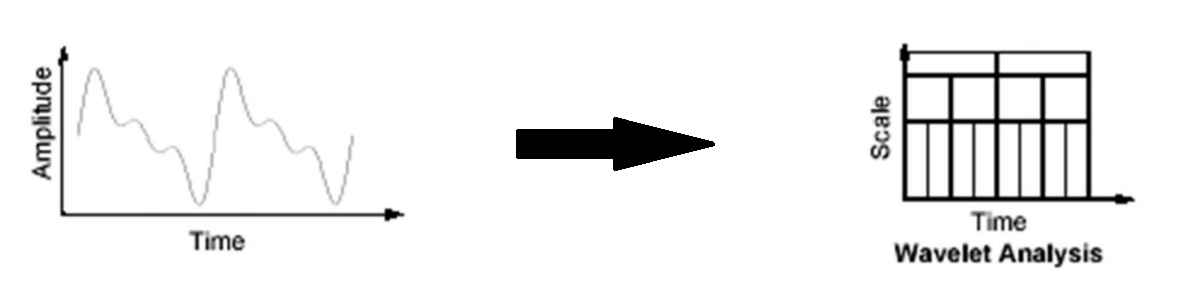
\includegraphics[width=0.8\textwidth]{figures/signalToWavelet}
	\caption{Signal in the time domain to frequency domain using the wavelet transformation. Modified from C.Uvo.\cite{Uvo1995}}
	\label{fig:sigToWave}
\end{figure} \vspace{-.3cm}

The wavelet transform computes both the scale and time, where the scale being the information of the frequencies and the time being the location. The general form of the CWT is stated in equation \ref{eq:cwt}: 
%\begin{flalign}
%	C(s,p)=\int_{-\infty}^{\infty}f(t)\Psi (s,p) dt
%	\label{eq:wave}
%\end{flalign}

\begin{flalign}
	W(\tau,s) = \int_{-\infty}^{\infty} x(t)  \frac{1}{\sqrt{ \mid s \mid }} \psi *(\frac{t-\tau}{s})dt
	\label{eq:cwt}
\end{flalign}

Where $\psi *(\frac{\tau-t}{\s})$ is the wavelet and $x(\tau)$ is the signal time series.\cite{Uvo1995,Conraria2011}
To achieve the CWT, the signal is convoluted with the wavelet to get the wavelet coefficient $W$ for the specific time $\tau$ and frequency $s$. The wavelet coefficient represents the magnitude. 

This is done by computing the wavelet of the signal which then is compared to the wavelet for a section at the beginning of the signal. Then the coefficients for the specific frequency and time is calculated for the section of the signal. The wavelet is shifted to the right and repeated until the entire signal is covered. Then the wavelet is scaled and the coefficients is computed for the entire signal again for all frequencies.\cite{Uvo1995}

Different wavelets can be used to compute the wavelet transformation. In this study the Morlet wavelet is the used wavelet. 

The Morlet wavelet is one of the most common wavelets. This wavelet can be seen as analytic, because it has numerical properties and properties of simple conversion from scales to frequencies using equation \ref{eq:freqeq}.

\begin{flalign}
	f(s)=\frac{w_\psi}{2\pi s}
	\label{eq:freqeq}
\end{flalign}

Where $w_\psi$ denotes the central frequency properties of the wavelet.\cite{Conraria2011}

In MATLAB the cwt(x)-function can be used to compute the CWT by inserting the signal as input. By further defining the sampling frequency in the input, the frequency of the signal content will be displayed. This will give a scalogram as shown in  \figref{fig:scalogram}.\cite{mathworks2017} 
The frequencies in Hz are shown along the logarithmic y-axis if the sampling frequency is specified, else it will show the normalized frequency in cycles per sample. Along the x-axis is the time vector. The scalogram shows the magnitude of the signal to show how the frequency in the signal is distributed. A scale to see the size of the magnitude is also implied.
% An example of a scalogram is given in \figref{fig:scalogram}

\begin{figure}[H]
	\centering	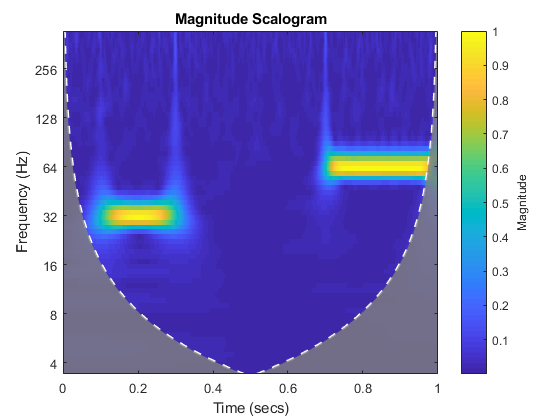
\includegraphics[width=0.65\textwidth]{figures/scalogram}
	\caption{An example of a scalogram, showing frequency content at 32 Hz at time approximately 0.2 s and 64 Hz at approximately 0.8 s.\cite{mathworks2017}}
	\label{fig:scalogram}
\end{figure} \vspace{-.3cm}

The signal of the wavelet is typically of a finite length, which sets some limitations to the CWT, like the edge effect. The edge effect is an expression of the lack of data, caused by truncation, to calculate specific frequencies because the lower frequencies have bigger windows and thereby reguire a bigger amount of data to be calculated.\cite{mari1999} The cone of influence (COI) shows the regions of the CWT where edge effects become significant. The gray zone are the areas where the edge effects become significant, which means that there will be some uncertainties to the CWT in this zone.\cite{mathworks2017}

%\begin{flalign}
%W(t,s) \equiv \int_{-\infty}^{\infty} \frac{1}{s^n} \psi *(\frac{\tau-t}{\s})x(\tau)d\tau
%\label{eq:cwt}
%\end{flalign}

%\begin{flalign}
%	W(t,s) = \frac{1}{2\pi} \int_{-\infty}^{\infty} \Psi*(s\omega)X(\omega)e^{i\omega t} d\omega
%	\label{eq:cwt2}
%\end{flalign}
